\chapter{Introduction}
Lipids are amphiphilic molecules, consisting of hydrophilic headgroup
and hydrophobic chains. There are various kinds of lipids. These can be 
categorized in terms of headgroup, chain length, and chain saturation.

In water lipids self-assemble into lipid bilayes to shield their hydrophobic 
cores. Lipid bilayers are the building blocks of cell membranes. Lipid bilayers 
display a wide variety of thermodynamic phases
as a function of temperature and hydration. Figure~\ref{fig:phase_diagram}
shows a generic phase diagram of phosphatidylcholines (PC).
At full hydration, a lamellar phase coexists with excess water.
PC lipids constitute a substantial fraction of mammalian cell membranes
and have been studied for many decades.
In the high temperature, fluid L$_\alpha$ phase, the hydrocarbon chains 
are conformationally disordered, and intra-membrane molecular correlations 
are liquid-like \cite{ref:Fahey78}. In the low temperature, gel L$_\beta'$
phase, hydrocarbon chains are stiff and titled with respect to the membrane
normal \cite{ref:Tardieu73}.
Between the fluid and gel phases appears a structurally modulated or 
rippled membrane phase. This phase has been detected in several 
lipids (REF: cite as many lipids as possible).
The low angle diffraction pattern of this phase conforms to the symmetry
of a 2D monoclinic lattice. This phase was termed P$_\beta'$ and is commonly
called the ripple phase. The topography of the membrane ripples has been directly
visualized by freeze fracture electron microscopy experiments 
\cite{ref:Luna77,ref:Copeland80,ref:Ruppel83,ref:Zasadzinski87,ref:Zasadzinski88}.
The wavelength of the modulation is about 140 \AA for dimyristoylphosphatidylcholine (DMPC),
which has 14 carbons in the hydro carbon chains \cite{ref:Wack89}.
There was evidence that molecular conformation in the ripple phase is not 
unique. NMR signals in the ripple phase \cite{ref:Wittebort81} were consistent
with a superposition of signals observed in the fluid and gel phases.
Lateral diffusion measurements found two distinct populations,
with diffusion coefficients characteristic of fluid and gel phases
\cite{ref:Schneider83}. 

At higher temperature, lipids are in fluid phase. In this phase, chains
are flexible. Lipid bilayers are also flexible and fluctuating. This
flexibility of lipid bilayers make many interesting biological
phenomena possible. 

\begin{figure}
  \centering
  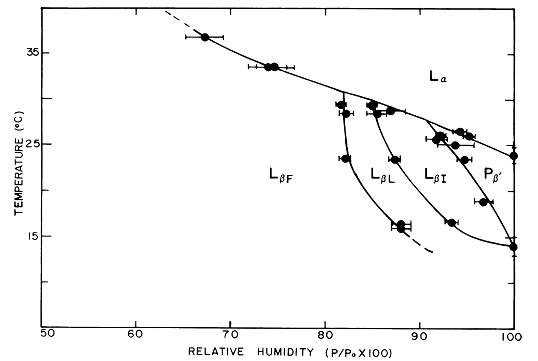
\includegraphics[width=0.9\textwidth]{figures/ripple/smith_phase_diagram}
  \caption{Experimental phase diagram of DMPC from Ref.~\cite{ref:Smith88}.}
  \label{fig:phase_diagram}
\end{figure}

As the temperature is reduced, lipid bilayers go into the gel phase.
In this phase, chains are straightened out and bilayers are rigid.

Between the fluid and gel phases, some lipids have the ripple phase.
This phase is found in saturated lipids. In this phase, the bilayer
height is modulated in a periodic manner in the in-plane direction.
Each bilayer is registered along its orthogonal direction.

In this thesis, we forcus on the fluid and ripple phase. In the former phase,
we investigated the interaction of a peptide called Tat with lipid bilayers
in the fluid phase. 
Tat is discussed in chapter 3.
Regarding the ripple phase, we measured the electron density profile of the lipid
bilayers using a stack of oriented bilayers. Using wide angle x-ray scattering
technique, we also investigated the chain packing within a bilayer. 
The ripple phase is discussed in chapter 4. 
The appendices show a lot of details that will
allow other people to reproduce much of the results shown in this thesis 
as well as help readers understand scattering analysis employed in this work.
It is my hope that these details will help future researchers,
especially students, understand some of the techniques to investigate the
structure of lipid bilayers in sub Angstrom resolution.